\section{Einachsiger Spannungszustand\label{spannung:section:Einachsiger Spannungsustand}}
\rhead{Einachsiger Spannungszustand}
Ein Spannungszustand beschreibt alle Spannungen, welche in einem beliebigen Punkt im Körper wirken (siehe Abbildung 1.4).
Änderungen der äusseren Kräfte verändern die inneren Spannungszustände im Material.
Um alle Spannungen eines Punktes darstellen zu können, wird ein infinitesimales Bodenelement in Form eines Würfels modellhaft vorgestellt.
Man spricht auch von einem Elementarwürfel, da dieser elementar klein ist.

\begin{figure}
	\centering
	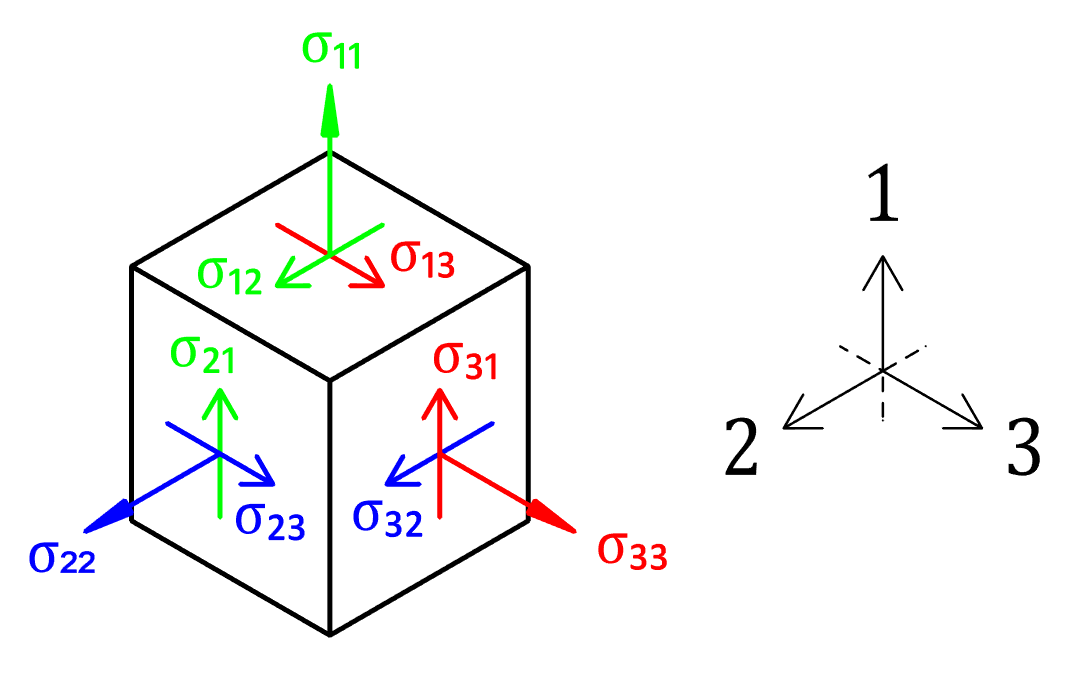
\includegraphics[width=0.5\linewidth,keepaspectratio]{papers/spannung/Grafiken/Bild2.png}
	\caption{Infinitesimales Bodenelement mit den 9 Spannungen}
	\label{fig:infintesimaler-wurfel}
\end{figure}

Es werden jeweils drei Seiten dieses Würfels betrachtet, wobei die drei gegenüberliegenden Seiten die selben Spannungen aufweisen.
Das infinitesimale Bodenteilchen hat die Koordinaten $1$, $2$, $3$ muss sich zwingend im Gleichgewicht befinden.
So sind insgesamt 9 verschiedene Spannungen möglich, wobei 3 Normal- und 6 Schubspannungen sind.
Normalspannung wirken normal (mit rechtem Winkel) zur angreifenden Fläche und Schubspannungen parallel zur angreifenden Fläche.
Alle Beträge dieser 9 Spannungen am Elementarwürfel bilden den Spannungszustand.
Daraus können die äquivalenten Dehnungen $\varepsilon$ mit Hilfe des Hook'schen Gesetz berechnet werden.

\begin{figure}
	\centering
	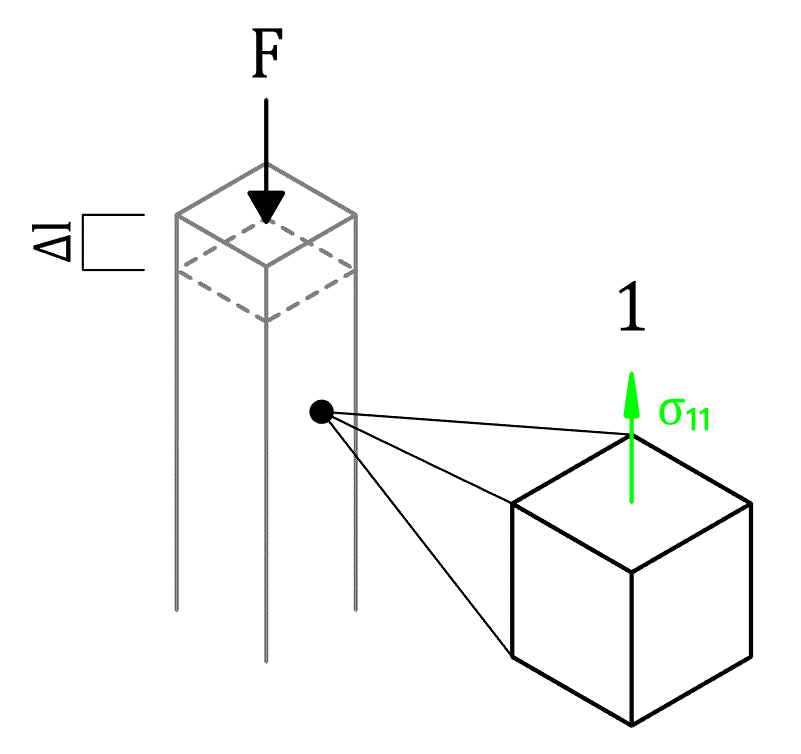
\includegraphics[width=0.5\linewidth,keepaspectratio]{papers/spannung/Grafiken/Bild1.png}
	\caption{1D Spannungszustand aus einer quaderförmigen Bodenprobe}
	\label{fig:infintesimaler-wurfel}
\end{figure}

Im einachsigen Spannungszustand herrscht nur die Normalspannung $\sigma_{11}$ (siehe Abbildung).
Das Hook'sche Gesetz beschreibt genau diesen 1D Spannungszustand.
Nach Hooke gilt:
\[
F
\sim
\Delta l
\]
.
Teilt man beide Seiten mit den Konstanten $A$ und $l_0$ erhält man
\[
\frac{F}{A}
=
\sigma
\sim
\]
\[
\varepsilon
=
\frac{\Delta l}{l_0}
\]
und somit
\[
\sigma
\sim
\varepsilon
\]
.
Mit:
\[
l_0
=
\text{Länge zu Beginn [\si{\meter}]}
\]
\[
A
=
\text{Fläche [\si{\meter\squared}]}
\]

Diese Beziehung gilt bei linear elastischen Materialien, welche reversibel sind und nicht dauerhaft verformt werden.
Es ist praktisch die relative Dehnung $\varepsilon$ anzugeben und nicht eine absolute Längenänderung $\Delta l$.
Mithilfe vom Elastizitätsmodul $E$ als Proportionalitätskonstante lässt sich der eindimensionale Fall mit
\[
\sigma
=
E\cdot\varepsilon
\]
beschreiben.
Im Falle, dass der E-Modul nicht konstant ist, kann dieser näherungsweise mit
\[
E
=
\frac{\Delta\sigma}{\Delta\varepsilon}
\]
ausgedrückt werden.